\item En un estudio realizado con 900 profesionales, 25 años después de su graduación, se descubre que 300 de ellos tuvieron éxito profesional, 300 de ellos se radicaron en el extranjero y 100 de ellos tuvieron éxito y se radicaron en el extranjero. Hallar el número de personas en el grupo que de estas dos cosas hayan hecho:
    \begin{enumerate}
        \item exactamente dos.\e\\
            Si se consideran los eventos
            \begin{center}
                $A=$ es exitoso\\
                $B=$ radicado en el extranjero 
            \end{center}
            es posible realizar el siguiente diagrama de Venn
            \begin{center}
                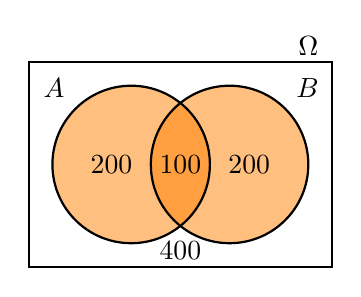
\begin{tikzpicture}[thick,
                    set/.style = {circle,
                                minimum size = 2cm,
                                fill=orange,
                                opacity=0.5}]
                    \draw [draw=black] (-1.3,-1.3) rectangle (2.55,1.3);
                    % Set A
                    \node[set,label={135:$A$}] (A) at (0,0) {};
                    % Set B
                    \node[set,label={45:$B$}] (B) at (1.25,0) {};
                    % Circles outline
                    \draw (0,0) circle(1cm);
                    \draw (1.25,0) circle(1cm);
                    % Set intersection label
                    \node at (0.625,0) {100};
                    \node at (-0.25,0) {200};
                    \node at (1.5,0) {200};
                    \node at (0.625,-1.1) {400};
                    \node at (2.25,1.5) {$\Omega$};
                \end{tikzpicture}
            \end{center}
            Hay 100 personas que son exitosas y están radicadas en el extranjero
        \item por lo menos una.\e\\
            En el diagrama podemos ver que hay 400 personas que no lograron ninguna de las dos, así que son $500(=900-400)$ aquellas que al menos lograron una.\e
        \item no más de una.\e\\
            Este grupo está conformado por las 200 personas que son exitosas pero no están en el extranjero y por las 200 personas radicadas en el extranjero pero no exitosas. Por lo tanto, hay 400 personas en total.
    \end{enumerate}